\section{Act III}

\begin{center}
	\begin{tikzpicture}[s/.style = {draw, rectangle}]
		\node[s] (n1) {\inlinegraphics{Assets/wp} Kurast Docks};

		%---- -1
		\node[s] (n2) at (0, -1) {\inlinegraphics{Assets/wp} Spider Forest};

		\draw[->] (n1) -- (n2);

		%---- -2
		\node[s,gray] (n3) at (-6, -2) {Arachnid Lair};
		\node[s] (n4) at (6, -2) {\inlinegraphics{Assets/Q3} Spider Cavern};

		\draw[->,gray] (n2.south) |- ($(n2.south) - (0, 2mm)$) -| (n3.north);
		\draw[->] (n2.south) |- ($(n2.south) - (0, 2mm)$) -| (n4.north);

		%---- -3
		\node[s,gray] (n5) at (-6, -3) {\inlinegraphics{Assets/wp} Great Marsh};

		\draw[->,gray] (n2.south) |- ($(n2.south) - (0, 11.5mm)$) -| (n5.north);

		%---- -4
		\node[s] (n6) at (0, -4) {\inlinegraphics{Assets/wp}\inlinegraphics{Assets/Q2} Flayer Jungle};

		\draw[->,gray] (n5.south) |- ($(n5.south) - (0, 2mm)$) -| (n6.north);
		\draw[->] (n2) -- (n6);

		%---- -5
		\node[s,gray] (n7) at (-6, -5) {Swampy Pit - Level 1};
		\node[s] (n8) at (6, -5) {Flayer Dungeon - Level 1};

		\draw[->,gray] (n6.south) |- ($(n6.south) - (0, 2.5mm)$) -| (n7.north);
		\draw[->] (n6.south) |- ($(n6.south) - (0, 2.5mm)$) -| (n8.north);

		%---- -6.5
		\node[s,gray] (n9) at (-6, -6.5) {Swampy Pit - Level 2};
		\node[s] (n10) at (6, -6.5) {Flayer Dungeon - Level 2};

		\draw[->,gray] (n7) -- (n9) node[midway, right] {Left};
		\draw[->] (n8) -- (n10) node[midway, left] {Left};

		%---- -8
		\node[s,gray] (n11) at (-6, -8) {Swampy Pit - Level 3};
		\node[s] (n12) at (6, -8) {\inlinegraphics{Assets/Q3} \internallink{MapsActIIIFlayerDungeonLevel3}{Flayer Dungeon - Level 3}};
		\node[s] (n13) at (0, -8) {\inlinegraphics{Assets/wp} Lower Kurast};

		\draw[->,gray] (n9) -- (n11) node[midway, right] {Left};
		\draw[->] (n10) -- (n12) node[midway, left] {Left};
		\draw[->] (n6) -- (n13);

		%---- -9
		\node[s] (n14) at (0, -9) {\inlinegraphics{Assets/wp} Kurast Bazaar};

		\draw[->] (n13) -- (n14);

		%---- -10.495
		\node[s,gray] (n15) at (-6, -10.495) {Disused Fane};
		\node[s] (n16) at (6, -10.495) {\inlinegraphics{Assets/Q4} Ruined Temple};

		\draw[->,gray] (n14.south) |- ($(n14.south) - (0, 7.5mm)$) -| (n15.north);
		\draw[->] (n14.south) |- ($(n14.south) - (0, 7.5mm)$) -| (n16.north) node[near start,above] {Entrance facing South West};

		%---- -11.5
		\node[s] (n17) at (6, -11.5) {Sewers - Level 1};

		\draw[->] (n14.south) |- ($(n14.south) - (0, 17.5mm)$) -| (n17.north);

		%---- -13
		\node[s] (n18) at (0, -13) {\inlinegraphics{Assets/wp} Upper Kurast};
		\node[s] (n19) at (6, -13) {\inlinegraphics{Assets/Q3} Sewers - Level 2};

		\draw[->] (n14) -- (n18);
		\draw[->] (n17) -- (n19) node[midway, left] {Right from Chest};

		%---- -14
		\node[s,gray] (n20) at (-6, -14) {Forgotten Temple};

		\draw[->,gray] (n18.south) |- ($(n18.south) - (0, 2mm)$) -| (n20.north);

		%---- -15
		\node[s,gray] (n21) at (-6, -15) {Forgotten Reliquary};
		\node[s] (n22) at (0, -15) {Kurast Causeway};

		\draw[->,gray] (n18.south) |- ($(n18.south) - (0, 11.5mm)$) -| (n21.north);
		\draw[->] (n18) -- (n22);

		%---- -16
		\node[s,gray] (n23) at (-6, -16) {Disused Reliquary};

		\draw[->,gray] (n22.south) |- ($(n22.south) - (0, 2mm)$) -| (n23.north);

		%---- -17
		\node[s,gray] (n23) at (-6, -17) {Ruined Fane};
		\node[s] (n24) at (0, -17) {\inlinegraphics{Assets/wp}\inlinegraphics{Assets/Q3}\inlinegraphics{Assets/Q5} Travincal};

		\draw[->,gray] (n22.south) |- ($(n22.south) - (0, 11.5mm)$) -| (n23.north);
		\draw[->] (n22) -- (n24);

		%---- -18
		\node[s] (n25) at (0, -18) {Durance of Hate - Level 1};

		\draw[->] (n24) -- (n25);

		%---- -19.5
		\node[s] (n26) at (0, -19.5) {\inlinegraphics{Assets/wp} Durance of Hate - Level 2};
		\node (e1) at (3.2, -19.5) {WP Left};

		\draw[->] (n25) -- (n26) node[midway, right] {Left};

		%---- -21
		\node[s] (n27) at (0, -21.5) {\inlinegraphics{Assets/Q6} Durance of Hate - Level 3};

		\draw[->] (n26) -- (n27) node[midway, right, text width=3cm] {Straight,\\Left from WP};
	\end{tikzpicture}
\end{center}

\clearpage
\subsection{Notes}

\subsubsection{\internallinkicon Flayer Dungeon - Level 3}\label{MapsActIIIFlayerDungeonLevel3}

Navigation: 6 set maps exist. Look at the images in Figure \ref{Figure:MapsActIIFlayerDungeonLevel3}.


\begin{figure}
	\centering
	\begin{subfigure}{0.495\hsize}
		\centering
		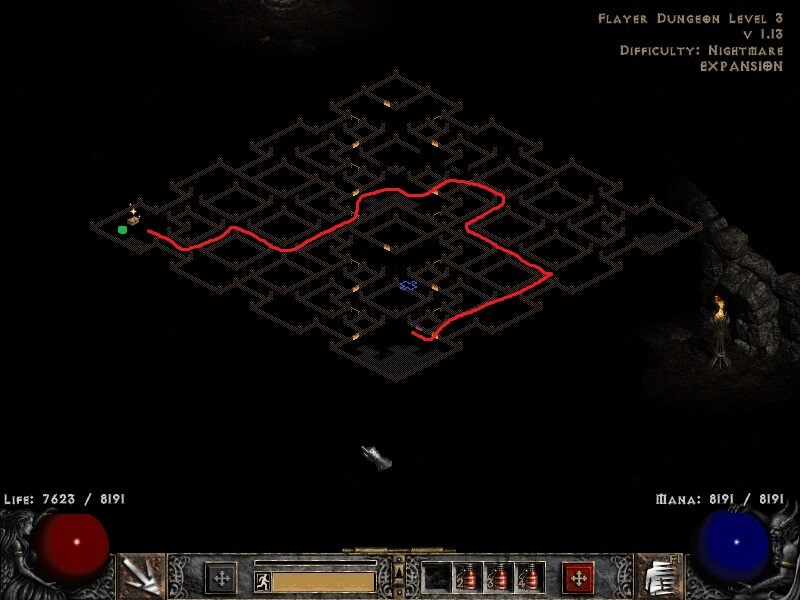
\includegraphics[width=\hsize]{Assets/FlayerDungeon3_1}
	\end{subfigure}
	\hfill
	\begin{subfigure}{0.495\hsize}
		\centering
		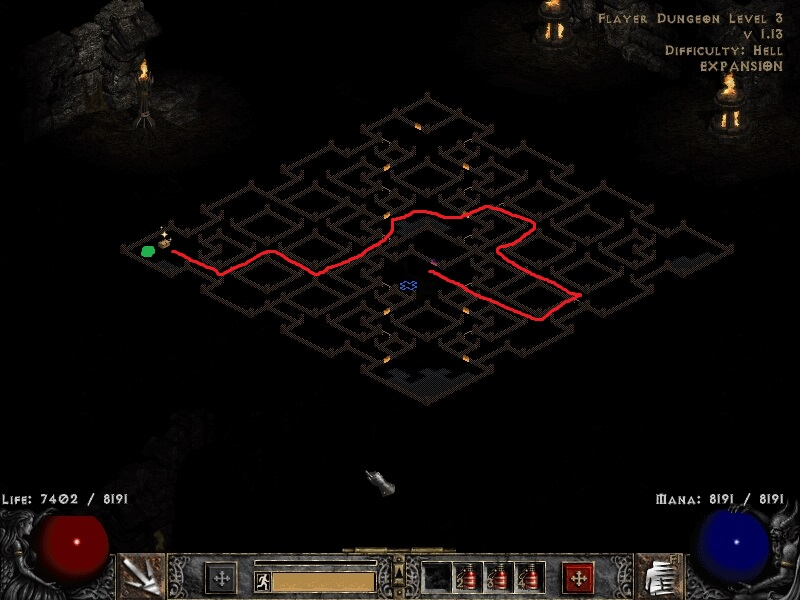
\includegraphics[width=\hsize]{Assets/FlayerDungeon3_2}
	\end{subfigure}

	\medskip
	\begin{subfigure}{0.495\hsize}
		\centering
		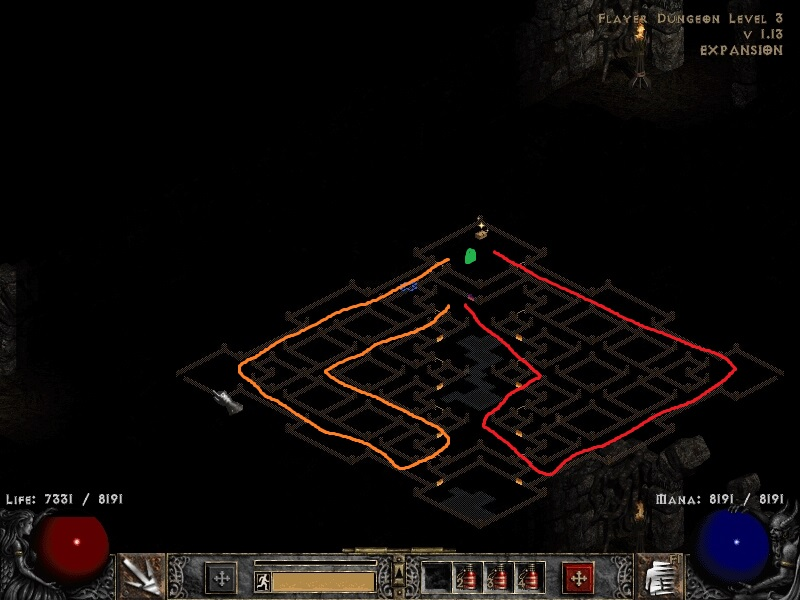
\includegraphics[width=\hsize]{Assets/FlayerDungeon3_3}
	\end{subfigure}
	\hfill
	\begin{subfigure}{0.495\hsize}
		\centering
		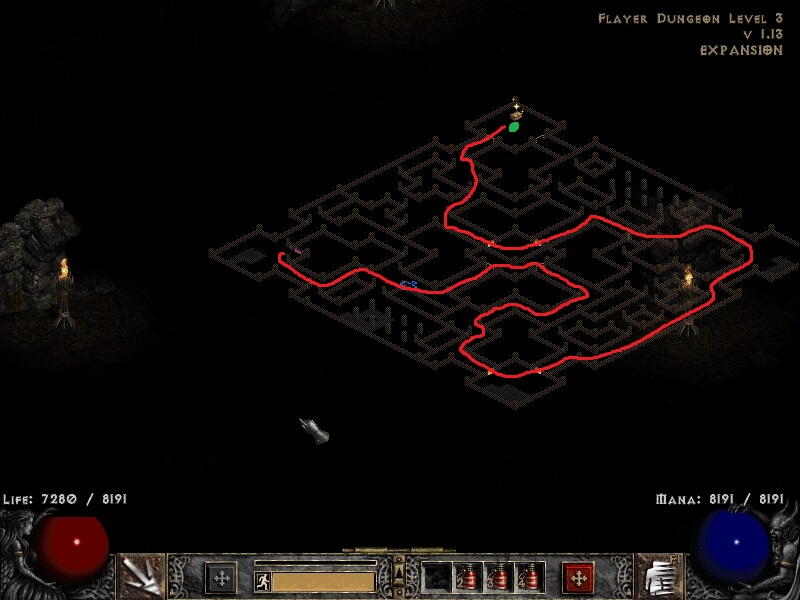
\includegraphics[width=\hsize]{Assets/FlayerDungeon3_4}
	\end{subfigure}

	\medskip
	\begin{subfigure}{0.495\hsize}
		\centering
		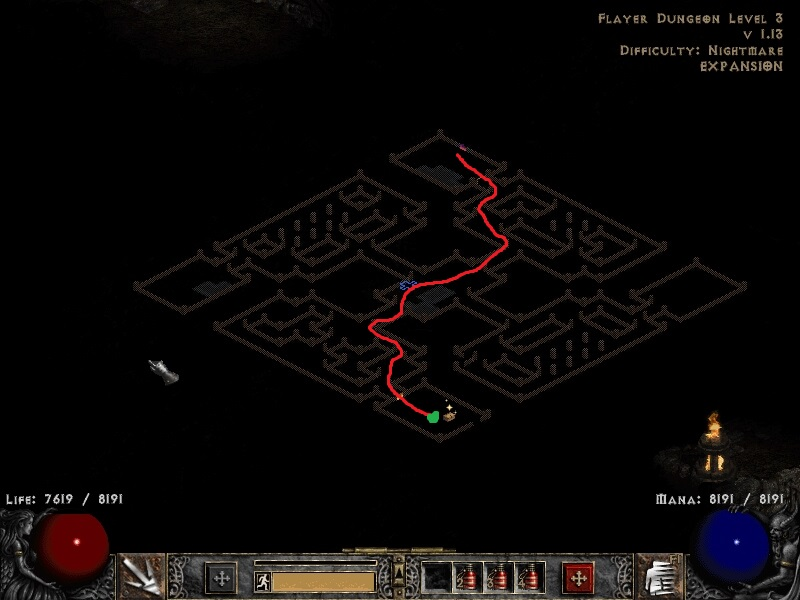
\includegraphics[width=\hsize]{Assets/FlayerDungeon3_5}
	\end{subfigure}
	\hfill
	\begin{subfigure}{0.495\hsize}
		\centering
		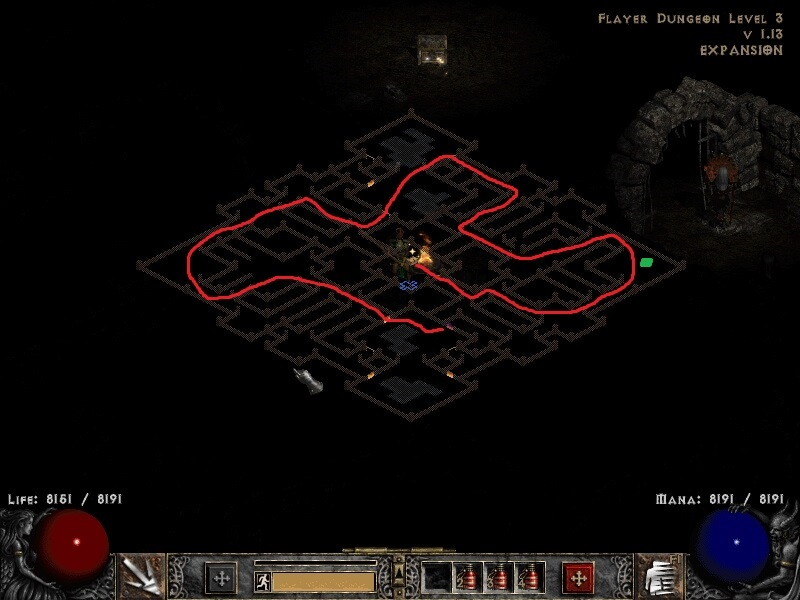
\includegraphics[width=\hsize]{Assets/FlayerDungeon3_6}
	\end{subfigure}
	\caption{Possible Flayer Dungeon - Level 3 maps\cite{flayerdungeon3maps}}
	\label{Figure:MapsActIIFlayerDungeonLevel3}
\end{figure}
